%To compile as handout, use
%pdflatex "\def\ishandout{1} \input{filename.tex}"
%Defaults to non-handout mode (with slide reveals)
\ifdefined\ishandout
  \documentclass[handout]{beamer}
\else
  \documentclass{beamer}
\fi
 
\usepackage{econ103slides} 

\date{Lecture \# 12}
\begin{document} 

%%%%%%%%%%%%%%%%%%%%%%%%%%%%%%%%%%%%%%%%

\begin{frame}[plain]
	\titlepage 
	

\end{frame} 

%%%%%%%%%%%%%%%%%%%%%%%%%%%%%%%%%%%%%%%%
\begin{frame}
  \frametitle{Continuous RVs II: The Normal RV}
\begin{figure}
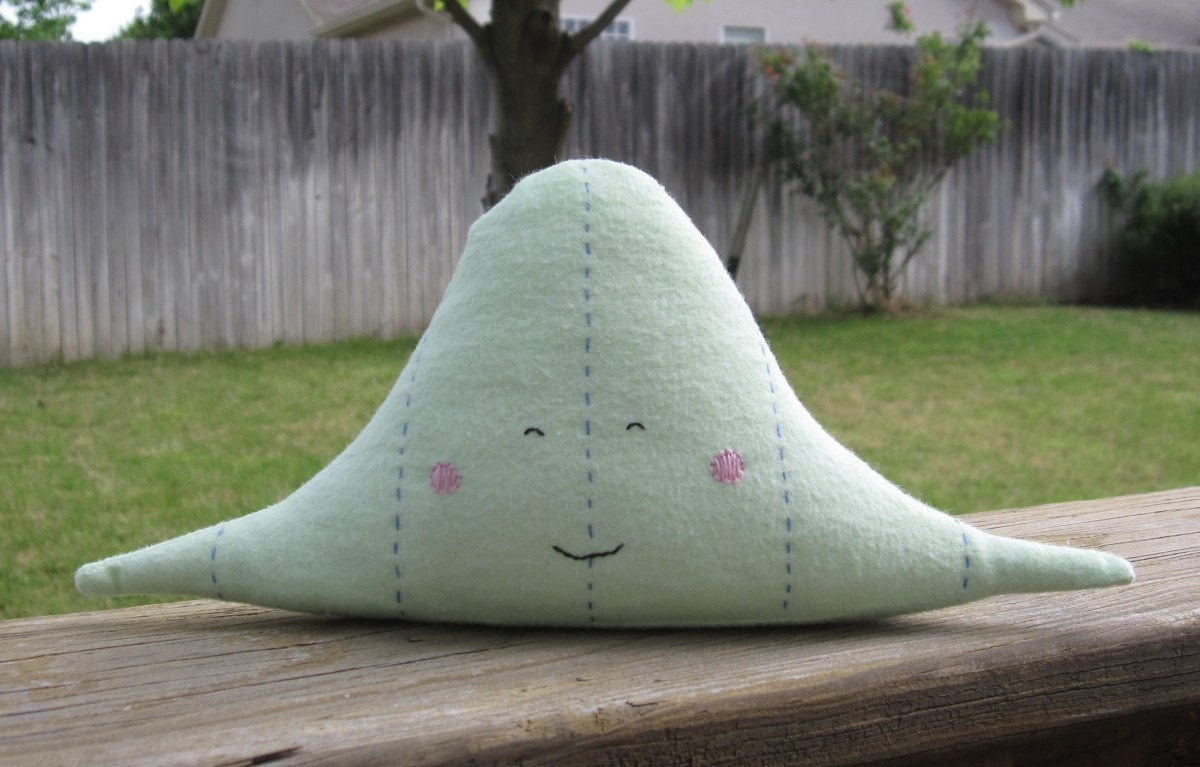
\includegraphics[scale = 0.2]{./images/normal_etsy1}
\caption{Standard Normal Distribution (PDF)}
\end{figure}
\end{frame}

%%%%%%%%%%%%%%%%%%%%%%%%%%%%%%%%%%%%%%%%
\begin{frame}
\frametitle{Standard Normal Random Variable: $N(0,1)$}

\begin{figure}[h]
  \centering
  \begin{tabular}{cc}
  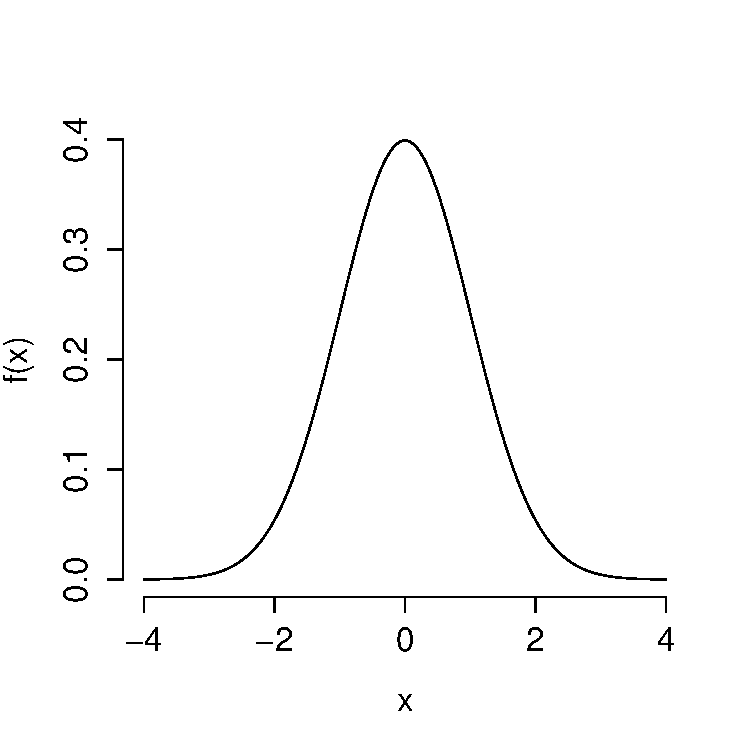
\includegraphics[scale = 0.3]{./images/std_normal_PDF}
  &  
  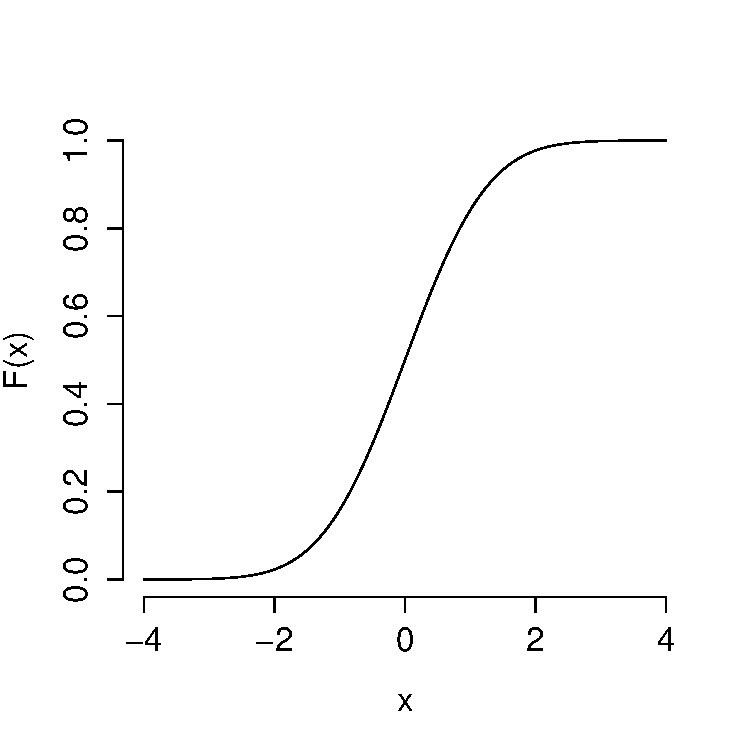
\includegraphics[scale = 0.3]{./images/std_normal_CDF}
\end{tabular}
\caption{Standard Normal PDF (left) and CDF (Right)}
\end{figure}
\begin{itemize}
  \item Notation: $X \sim N(0,1)$
  \item Symmetric, Bell-shaped, $E[X]=0$, $Var[X]=1$
  \item Support Set $= (-\infty,\infty)$
\end{itemize}
\end{frame}

%%%%%%%%%%%%%%%%%%%%%%%%%%%%%%%%%%%%%%%%

\begin{frame}
	\frametitle{\href{http://glimmer.rstudio.com/fditraglia/normal_cdf/}{http://glimmer.rstudio.com/fditraglia/normal\_cdf/}}

\begin{figure}
	\fbox{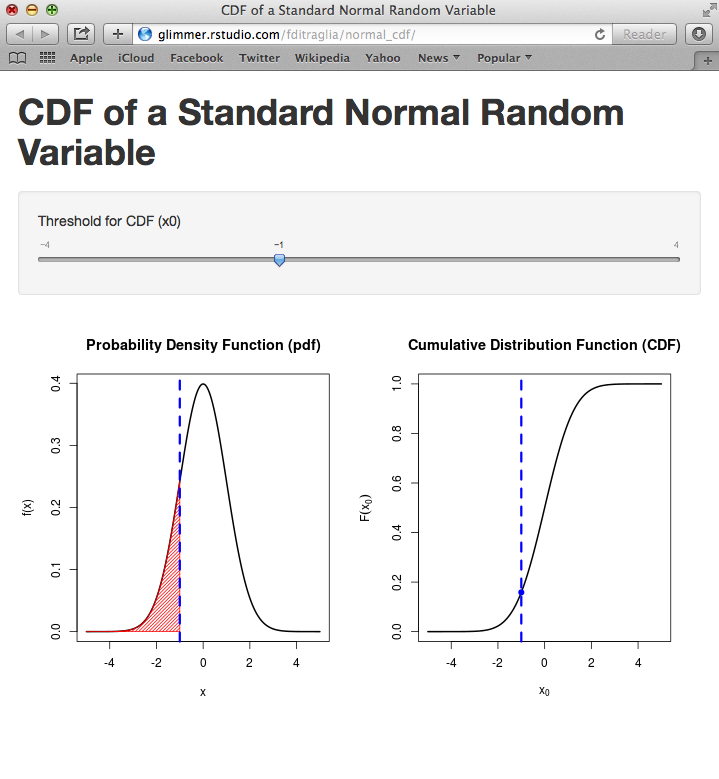
\includegraphics[scale = 0.2]{./images/normal_cdf_screenshot}}
\end{figure}

\end{frame}

%%%%%%%%%%%%%%%%%%%%%%%%%%%%%%%%%%%%%%%%
\begin{frame}
  \frametitle{Standard Normal Distribution: $N(0,1)$}
\begin{figure}[h]
  \centering
  \begin{tabular}{cc}
  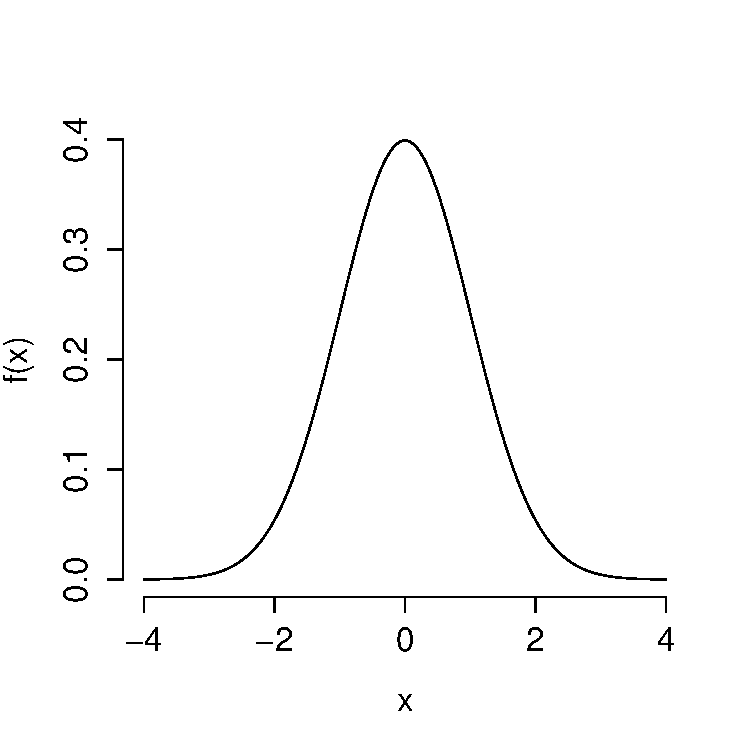
\includegraphics[scale = 0.3]{./images/std_normal_PDF}
  &  
  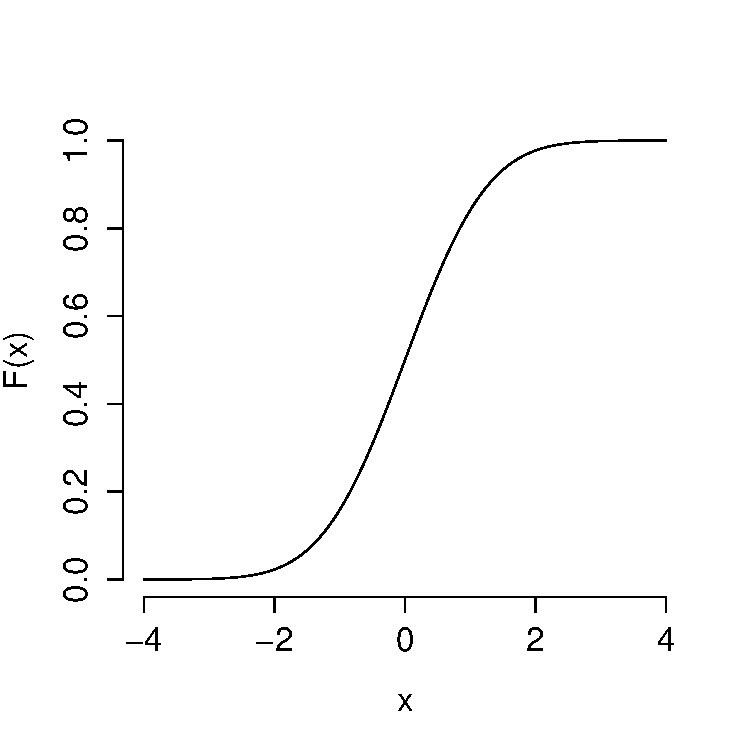
\includegraphics[scale = 0.3]{./images/std_normal_CDF}
\end{tabular}
\end{figure}
\begin{itemize}
  \item There is no closed-form expression for the $N(0,1)$ CDF.
  \item For Econ 103, don't need to know formula for $N(0,1)$ PDF.
  \item You \emph{do need} to know the R commands\dots
\end{itemize}
\end{frame}
%%%%%%%%%%%%%%%%%%%%%%%%%%%%%%%%%%%%%%%%
\begin{frame}
  \frametitle{R Commands for the Standard Normal RV}
  \begin{block}{\texttt{dnorm} -- \small Standard Normal PDF}
    \begin{itemize}
      \item Mnemonic: \texttt{d} $=$ density, \texttt{norm} $=$ normal
      \item Example: \texttt{dnorm(0)} gives height of $N(0,1)$ PDF at zero.
    \end{itemize}
  \end{block}
  \pause
  \begin{block}{\texttt{pnorm} -- \small Standard Normal CDF}
    \begin{itemize}
      \item Mnemonic: \texttt{p} $=$ probability, \texttt{norm} $=$ normal
      \item Example: $\texttt{pnorm(1)} = P(X\leq 1)$ if $X\sim N(0,1)$.
    \end{itemize}
  \end{block}
  \pause
  \begin{block}{\texttt{rnorm} -- \small Simulate Standard Normal Draws}
    \begin{itemize}
      \item Mnemonic: \texttt{r} $=$ random, \texttt{norm} $=$ normal. 
      \item Example: \texttt{rnorm(10)} makes ten iid $N(0,1)$ draws.
    \end{itemize}
  \end{block}
\end{frame}
%%%%%%%%%%%%%%%%%%%%%%%%%%%%%%%%%%%%%%%%
\begin{frame}
  \frametitle{$\Phi(x_0)$ Denotes the $N(0,1)$ CDF}
  You will sometimes encounter the notation $\Phi(x_0)$.
  It means the same thing as $\texttt{pnorm}(x_0)$ but it's not an R command. 
\end{frame}
%%%%%%%%%%%%%%%%%%%%%%%%%%%%%%%%%%%%%%%%
\begin{frame}
  \frametitle{The $N(\mu, \sigma^2)$ Random Variable}
  \begin{block}{Idea}
   Take a linear function of the $N(0,1)$ RV.
  \end{block}
  \begin{block}{Formal Definition}
    \alert{$N(\mu, \sigma^2) \equiv \mu + \sigma X$} where $X \sim N(0,1)$ and $\mu, \sigma$ are constants.
  \end{block}
  \begin{block}{Properties of $N(\mu, \sigma^2)$ RV}
    \begin{itemize}
      \item Parameters: Expected Value $= \mu$, Variance $= \sigma^2$
      \item Symmetric and bell-shaped. 
      \item Support Set $=(-\infty,\infty)$
      \item $N(0,1)$ is the special case where $\mu=0$ and $\sigma^2 = 1$. 
    \end{itemize}
  \end{block}
\end{frame}
%%%%%%%%%%%%%%%%%%%%%%%%%%%%%%%%%%%%%%%%
\begin{frame}
  \frametitle{Expected Value: $\mu$ \emph{shifts} PDF}
\framesubtitle{all of these have $\sigma=1$}

\begin{figure}
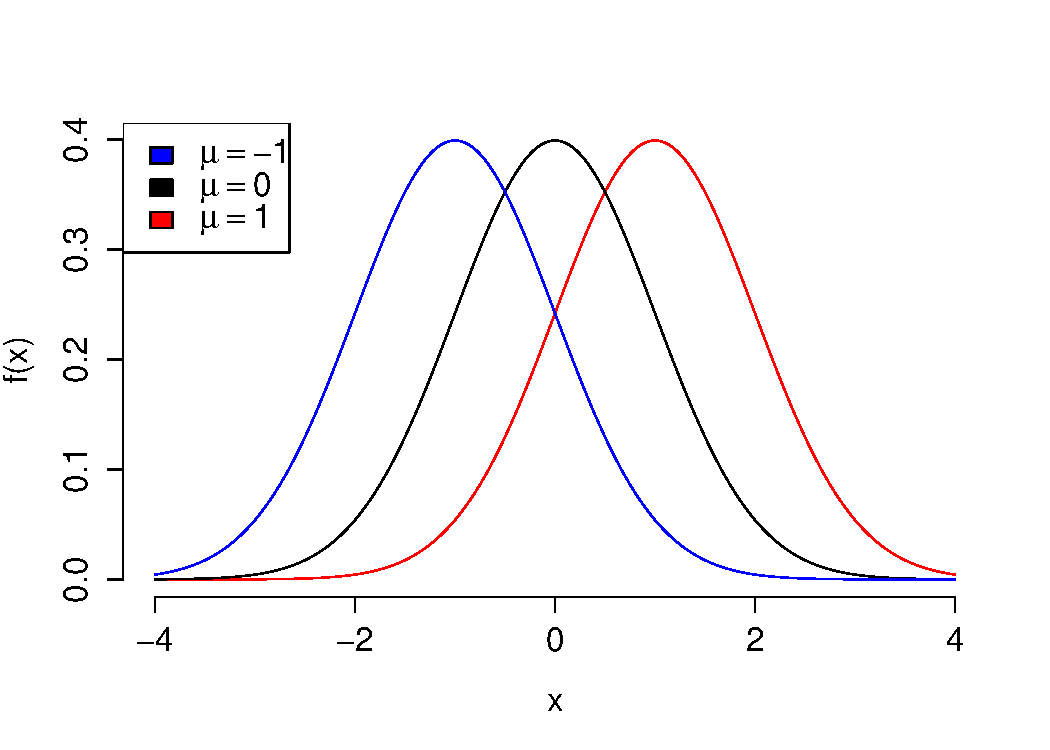
\includegraphics[scale = 0.5]{./images/normal_means}
\caption{\textcolor{blue}{Blue $\mu = -1$},
Black $\mu = 0$,
\textcolor{red}{Red $\mu = 1$}}
\end{figure}
\end{frame}

%%%%%%%%%%%%%%%%%%%%%%%%%%%%%%%%%%%%%%%%


\begin{frame}
  \frametitle{Standard Deviation: $\sigma$ \emph{scales} PDF}
\framesubtitle{all of these have $\mu=0$}

\begin{figure}
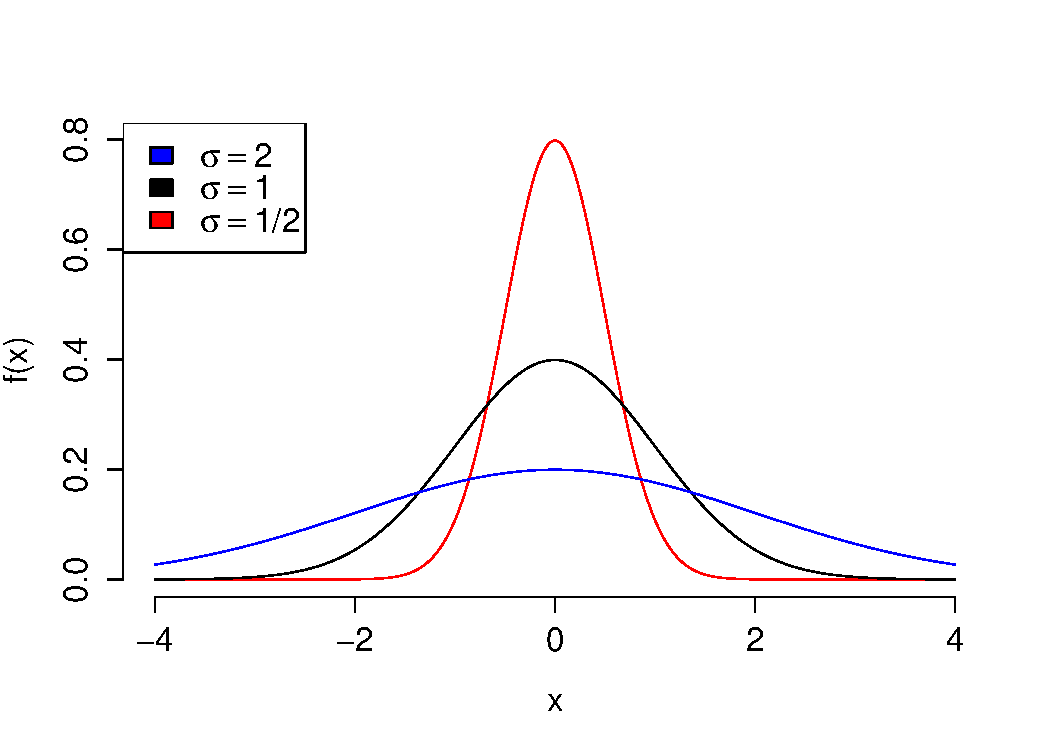
\includegraphics[scale = 0.5]{./images/normal_std_devs}
\caption{\textcolor{blue}{Blue $\sigma^2 = 4$},
Black $\sigma^2=1$,
\textcolor{red}{Red $\sigma^2= 1/4$}}
\end{figure}
\end{frame}

%%%%%%%%%%%%%%%%%%%%%%%%%%%%%%%%%%%%%%%%


\begin{frame}
\frametitle{Linear Function of Normal RV is a Normal RV}


Suppose that $X \sim N(\mu, \sigma^2)$. Then if $a$ and $b$ constants,
$$\boxed{a + bX \sim N(a + b\mu, b^2 \sigma^2)}$$

\begin{block}{Important}
	\begin{itemize}
    \item  For \emph{any} RV $X$, $E[a + bX] = a +bX$ and $Var(a +bX) = b^2 X$.
		\item Key point: linear transformation of normal is still normal!
    \item Linear transformation of Binomial is \emph{not} Binomial!
	\end{itemize}
\end{block}

\end{frame}

%%%%%%%%%%%%%%%%%%%%%%%%%%%%%%%%%%%%%%%%
\begin{frame}
\frametitle{Example \hfill 
\includegraphics[scale = 0.05]{./images/clicker}}
Suppose $X \sim N(\mu, \sigma^2)$ and let $Z = (X -\mu)/\sigma$. What is the distribution of $Z$?

\begin{enumerate}[(a)]
	\item $N(\mu, \sigma^2)$
	\item $N(\mu, \sigma)$
	\item $N(0, \sigma^2)$
	\item  $N(0, \sigma)$
	\item $N(0,1)$
\end{enumerate}
\end{frame}

%%%%%%%%%%%%%%%%%%%%%%%%%%%%%%%%%%%%%%%%
\begin{frame}
  \frametitle{Linear Combinations of \emph{Multiple Independent} Normals}
Let $X \sim N(\mu_x, \sigma^2_x)$ independent of $Y \sim N(\mu_y, \sigma^2_y)$. Then if $a,b,c$ are constants:

$$\boxed{aX + bY +c \sim N(a\mu_x + b\mu_y + c, a^2 \sigma_x^2 + b^2 \sigma_y^2)}$$



\begin{block}{Important}
	\begin{itemize}
		\item Result assumes independence
		\item Particular to Normal Distribution
		\item Extends to more than two Normal RVs
	\end{itemize}
\end{block}

\end{frame}
%%%%%%%%%%%%%%%%%%%%%%%%%%%%%%%%%%%%%%%%
\begin{frame}
\frametitle{Suppose $X_1, X_2, \sim \mbox{iid } N(\mu, \sigma^2)$ \hfill 
\includegraphics[scale = 0.05]{./images/clicker}}

Let $\bar{X} = (X_1 + X_2)/2$. What is the distribution of $\bar{X}$?
\begin{enumerate}[(a)]
\item $N(\mu, \sigma^2/2)$
\item $N(0,1)$
\item $N(\mu, \sigma^2)$
\item $N(\mu, 2\sigma^2)$
\item $N(2\mu, 2\sigma^2)$
\end{enumerate}

\end{frame}
%%%%%%%%%%%%%%%%%%%%%%%%%%%%%%%%%%%%%%%%
\begin{frame}
\frametitle{Where does the Empirical Rule come from?}

\begin{block}{Empirical Rule}
Approximately 68\% of observations within $\mu\pm \sigma$\\
Approximately 95\% of observations within $\mu\pm 2 \sigma$\\
Nearly all observations within $\mu\pm 3 \sigma$
\end{block}
\end{frame}

%%%%%%%%%%%%%%%%%%%%%%%%%%%%%%%%%%%%%%%%

\begin{frame}
\frametitle{\texttt{pnorm(1)}$\approx 0.84$}

\begin{figure}
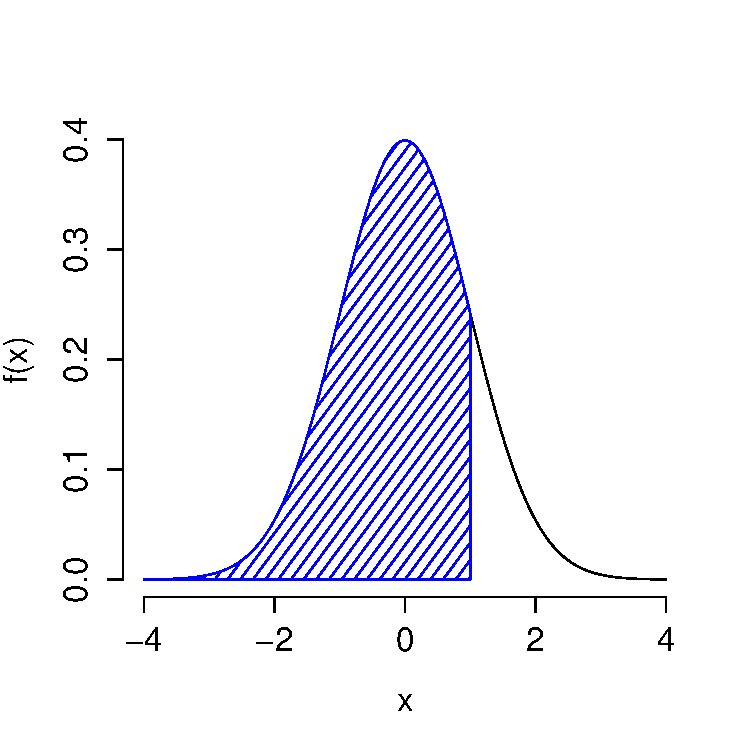
\includegraphics[scale = 0.65]{./images/middle68_1}
\end{figure}
\end{frame}
%%%%%%%%%%%%%%%%%%%%%%%%%%%%%%%%%%%%%%%%
\begin{frame}
\frametitle{\texttt{pnorm(1) - pnorm(-1)}$\approx 0.84 - 0.16$}
\begin{figure}
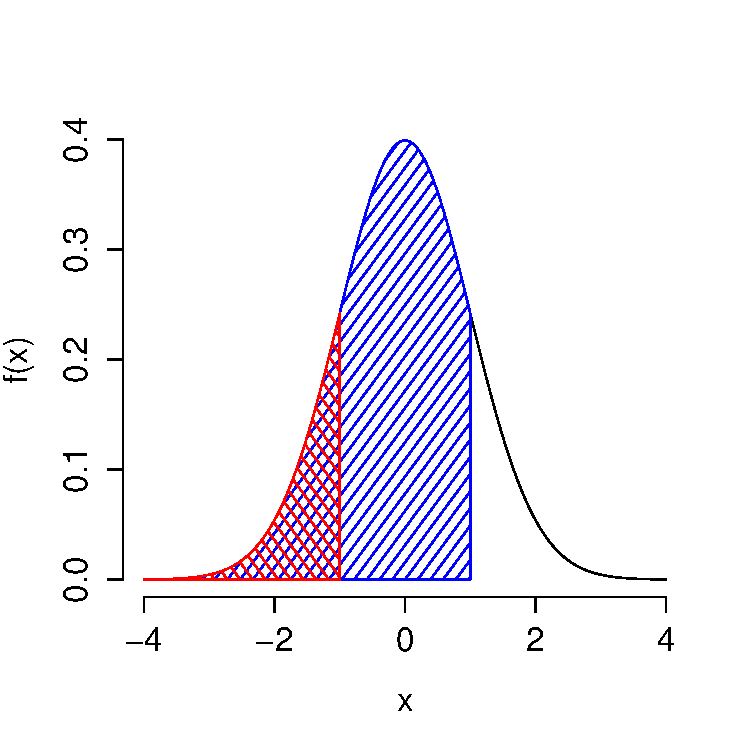
\includegraphics[scale = 0.65]{./images/middle68_2}
\end{figure}
\end{frame}
%%%%%%%%%%%%%%%%%%%%%%%%%%%%%%%%%%%%%%%%
\begin{frame}
\frametitle{\texttt{pnorm(1) - pnorm(-1)}$\approx 0.68$}
\begin{figure}
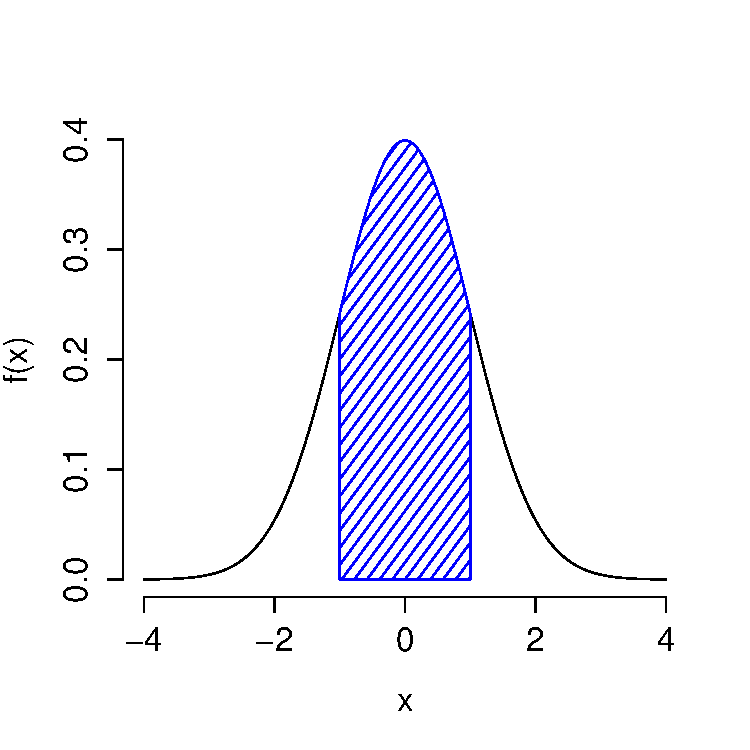
\includegraphics[scale = 0.65]{./images/middle68_3}
\end{figure}
\end{frame}
%%%%%%%%%%%%%%%%%%%%%%%%%%%%%%%%%%%%%%%%

\begin{frame}
\frametitle{Middle 68\% of $N(0,1) \Rightarrow$ approx.\ $(-1,1)$}
\begin{figure}
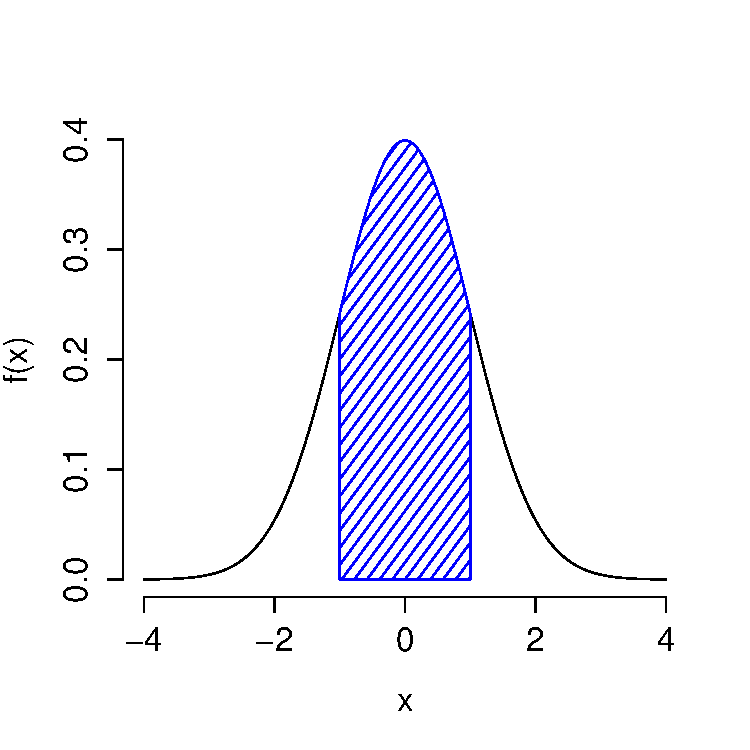
\includegraphics[scale = 0.65]{./images/normal_middle68}
\end{figure}
\end{frame}

%%%%%%%%%%%%%%%%%%%%%%%%%%%%%%%%%%%%%%%%
\begin{frame}
\frametitle{Suppose $X \sim N(0,1)$}
\begin{eqnarray*}
	P(-1 \leq X \leq 1) &=& \mbox{\texttt{pnorm(1) - pnorm(-1)}}\\
		&\approx& 0.683
\end{eqnarray*}
\begin{eqnarray*}
	P(-2 \leq X \leq 2) &=& \mbox{\texttt{pnorm(2) - pnorm(-2)}}\\
		&\approx& 0.954
\end{eqnarray*}
\begin{eqnarray*}
	P(-3 \leq X \leq 3) &=& \mbox{\texttt{pnorm(3) - pnorm(-3)}}\\
		&\approx& 0.997
\end{eqnarray*}

\end{frame}
%%%%%%%%%%%%%%%%%%%%%%%%%%%%%%%%%%%%%%%%
\begin{frame}
\frametitle{What if $X \sim N(\mu, \sigma^2)$?}
\begin{eqnarray*}
	P(X \leq a) &=& \pause P(X - \mu \leq a - \mu)\\\\
		&=& \pause P\left( \frac{X-\mu}{\sigma} \leq \frac{a - \mu}{\sigma} \right)\\\\
		&=&\pause  P\left(Z \leq  \frac{a - \mu}{\sigma}\right)
\end{eqnarray*}
Where $Z$ is a standard normal random variable, i.e.\ $N(0,1)$.
\end{frame}


%%%%%%%%%%%%%%%%%%%%%%%%%%%%%%%%%%%%%%%%
\begin{frame}
\frametitle{
\includegraphics[scale = 0.05]{./images/clicker}}
Which of these equals $P\left(Z \leq (a-\mu)/\sigma\right)$ if $Z\sim N(0,1)$?
	\begin{enumerate}[(a)]
    \item $\texttt{pnorm(a)}$
    \item $1 - \texttt{pnorm(a)}$
    \item $\texttt{pnorm(a)}/\sigma - \mu$
    \item $\texttt{pnorm}\left(\frac{a - \mu}{\sigma}  \right)$
		\item None of the above.
	\end{enumerate}
\end{frame}

%%%%%%%%%%%%%%%%%%%%%%%%%%%%%%%%%%%%%%%%
\begin{frame}
  \frametitle{Probability \emph{Above} a Threshold: $X \sim N(\mu, \sigma^2)$}
\begin{eqnarray*}
	P(X \geq b) &=&1 - P(X\leq b) =1 - P\left( \frac{X-\mu}{\sigma} \leq \frac{b-\mu}{\sigma} \right) \\ \\
	&=& 1 - P\left( Z \leq \frac{b-\mu}{\sigma} \right) \\
	&=& 1 -\mbox{\texttt{pnorm}}((b-\mu)/\sigma)
\end{eqnarray*}
Where $Z$ is a standard normal random variable.
\end{frame}
%%%%%%%%%%%%%%%%%%%%%%%%%%%%%%%%%%%%%%%%
\begin{frame}
\frametitle{Probability of an Interval: $X \sim N(\mu, \sigma^2)$}


\begin{eqnarray*}
	P(a \leq X \leq b) &=&  P\left( \frac{a - \mu}{\sigma} \leq \frac{X - \mu}{\sigma} \leq \frac{b-\mu}{\sigma} \right)\\ \\ 
	&=& P\left( \frac{a - \mu}{\sigma} \leq Z \leq \frac{b-\mu}{\sigma} \right)\\ \\ 
	&=&\ \mbox{\texttt{pnorm}}((b-\mu)/\sigma) -  \mbox{\texttt{pnorm}}((a-\mu)/\sigma)
\end{eqnarray*}
Where $Z$ is a standard normal random variable.
\end{frame}
%%%%%%%%%%%%%%%%%%%%%%%%%%%%%%%%%%%%%%%%
\begin{frame}
\frametitle{Suppose $X \sim N(\mu, \sigma^2)$\hfill 
\includegraphics[scale = 0.05]{./images/clicker}}
What is $P(\mu - \sigma \leq X \leq \mu + \sigma)$?

\pause
\begin{eqnarray*}
P(\mu - \sigma \leq X \leq \mu + \sigma) &=& P\left( -1 \leq \frac{X-\mu}{\sigma} \leq 1\right)\\ \\
	&=& P\left( -1 \leq Z \leq 1\right)\\
	&=& \mbox{\texttt{pnorm(1)}} -  \mbox{\texttt{pnorm(-1)}}\\
	&\approx& 0.68
\end{eqnarray*}
\end{frame}

%%%%%%%%%%%%%%%%%%%%%%%%%%%%%%%%%%%%%%%%

\begin{frame}
\frametitle{Percentiles/Quantiles for Continuous RVs}
\begin{block}{Quantile Function $Q(p)$ is the inverse of CDF $F(x_0)$}
Plug in a probability $p$, get out the value of $x_0$ such that $F(x_0)=p$
\end{block}
$$Q(p) = F^{-1}(p)$$

In other words:
	$$Q(p) = \mbox{the value of } x_0 \mbox{ such that } \int_{-\infty}^{x_0} f(x) \; dx = p$$
	
\begin{alertblock}{Inverse exists as long as $F(x_0)$ is \emph{strictly increasing}.} \end{alertblock}	
	
\end{frame}
%%%%%%%%%%%%%%%%%%%%%%%%%%%%%%%%%%%%%%%%
\begin{frame}
\frametitle{Example: Median}
The median of a continuous random variable is $Q(0.5)$, i.e.\ the value of $x_0$ such that 
	$$\int_{-\infty}^{x_0} f(x)\; dx = 1/2$$
\end{frame}
%%%%%%%%%%%%%%%%%%%%%%%%%%%%%%%%%%%%%%%%
\begin{frame}
\frametitle{What is the median of a standard normal RV?\hfill 
\includegraphics[scale = 0.05]{./images/clicker}}
\pause
By symmetry, $Q(0.5) = 0$. R command: \texttt{qnorm()}
\begin{center}
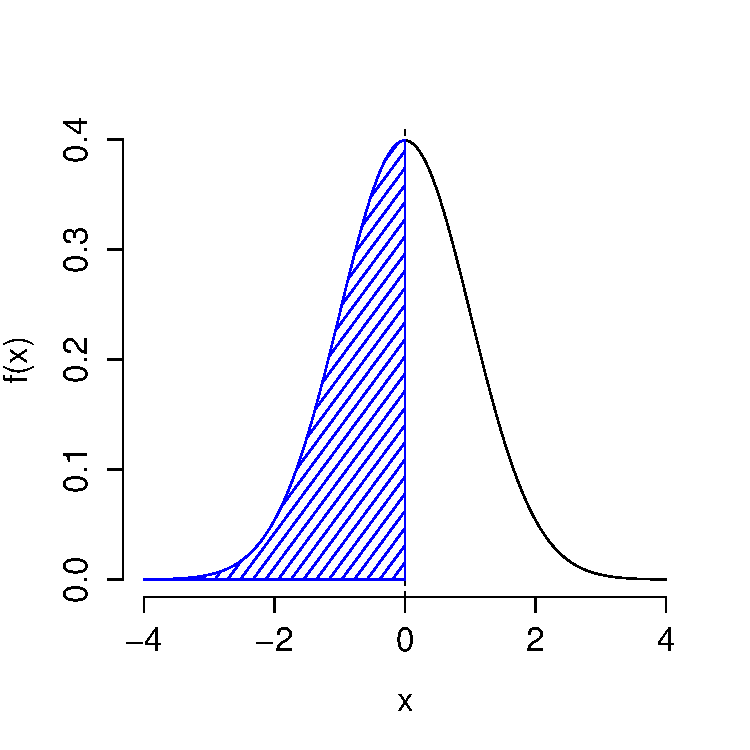
\includegraphics[scale = 0.6]{./images/normal_median}
\end{center}
\end{frame}
%%%%%%%%%%%%%%%%%%%%%%%%%%%%%%%%%%%%%%%%
\begin{frame}
\frametitle{90th Percentile of a Standard Normal}
\texttt{qnorm(0.9)}$\approx 1.28$
\begin{center}
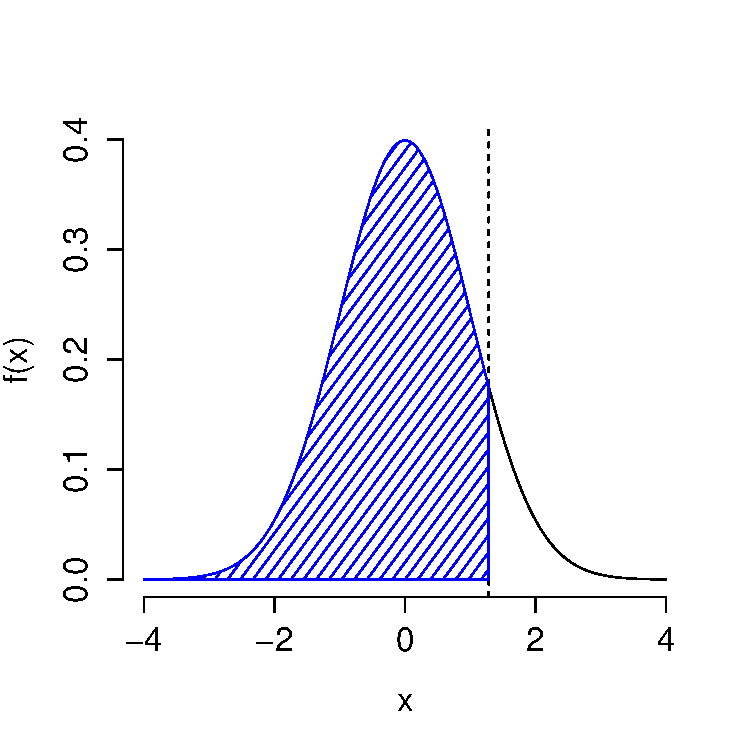
\includegraphics[scale = 0.6]{./images/normal90}
\end{center}
\end{frame}
%%%%%%%%%%%%%%%%%%%%%%%%%%%%%%%%%%%%%%%%

\begin{frame}
\frametitle{Using Quantile Function to find Symmetric Intervals}
Suppose $X$ is a standard normal RV. What is the value of $c$ such that $P(-c \leq X\leq c ) = 0.5$?
\begin{center}
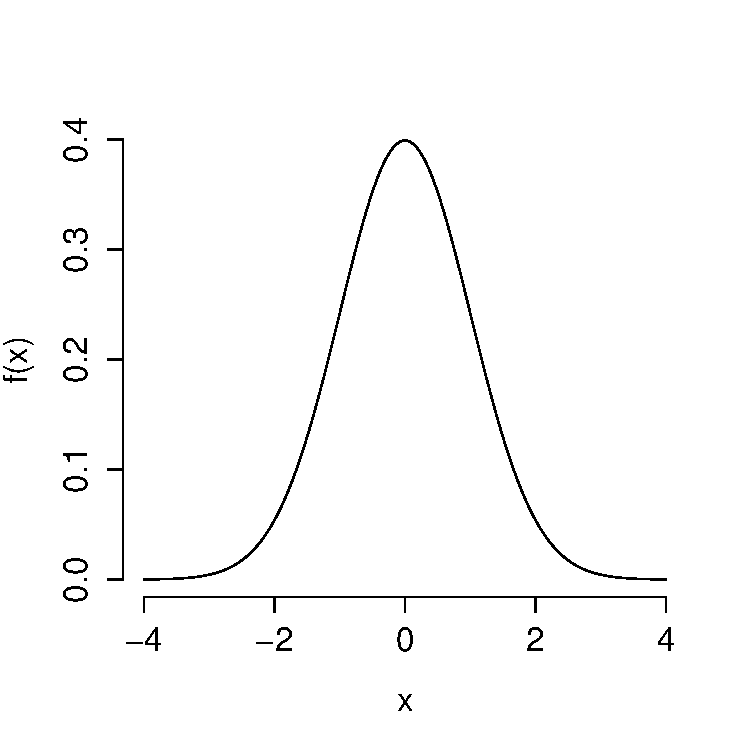
\includegraphics[scale = 0.55]{./images/tail1}
\end{center}
\end{frame}

%%%%%%%%%%%%%%%%%%%%%%%%%%%%%%%%%%%%%%%%
\begin{frame}
\frametitle{\texttt{qnorm(0.75)}$\approx 0.67$}
Suppose $X$ is a standard normal RV. What is the value of $c$ such that $P(-c \leq X\leq c ) = 0.5$?
\begin{center}
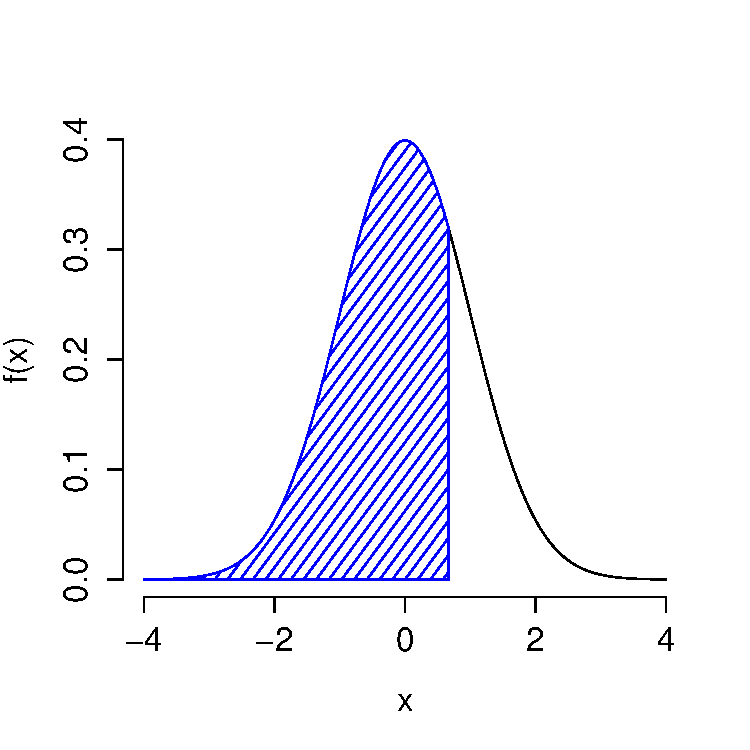
\includegraphics[scale = 0.55]{./images/tail2}
\end{center}
\end{frame}

%%%%%%%%%%%%%%%%%%%%%%%%%%%%%%%%%%%%%%%%
\begin{frame}
\frametitle{\texttt{qnorm(0.75)}$\approx 0.67$}
Suppose $X$ is a standard normal RV. What is the value of $c$ such that $P(-c \leq X\leq c ) = 0.5$?
\begin{center}
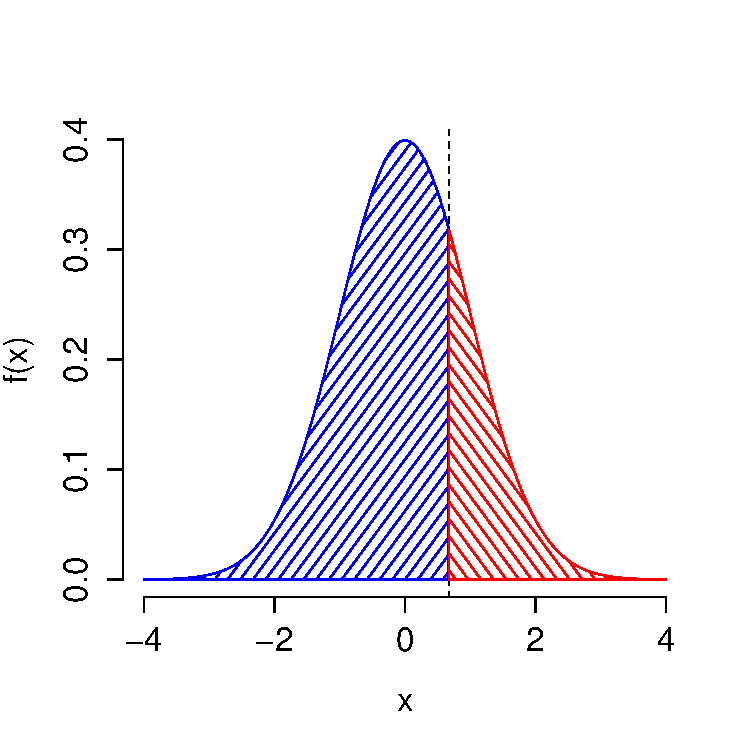
\includegraphics[scale = 0.55]{./images/tail3}
\end{center}
\end{frame}

%%%%%%%%%%%%%%%%%%%%%%%%%%%%%%%%%%%%%%%%

\begin{frame}
\frametitle{\texttt{pnorm(0.67)-pnorm(-0.67)}$\approx$?}
Suppose $X$ is a standard normal RV. What is the value of $c$ such that $P(-c \leq X\leq c ) = 0.5$?
\begin{center}
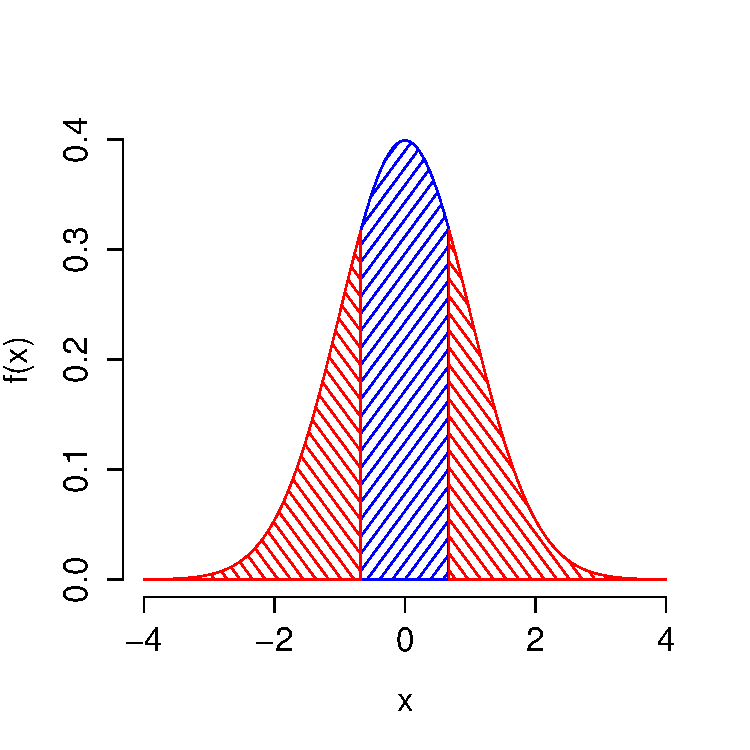
\includegraphics[scale = 0.55]{./images/tail4}
\end{center}
\end{frame}

%%%%%%%%%%%%%%%%%%%%%%%%%%%%%%%%%%%%%%%%


\begin{frame}
\frametitle{\texttt{pnorm(0.67)-pnorm(-0.67)}$\approx 0.5$}
Suppose $X$ is a standard normal RV. What is the value of $c$ such that $P(-c \leq X\leq c ) = 0.5$?
\begin{center}
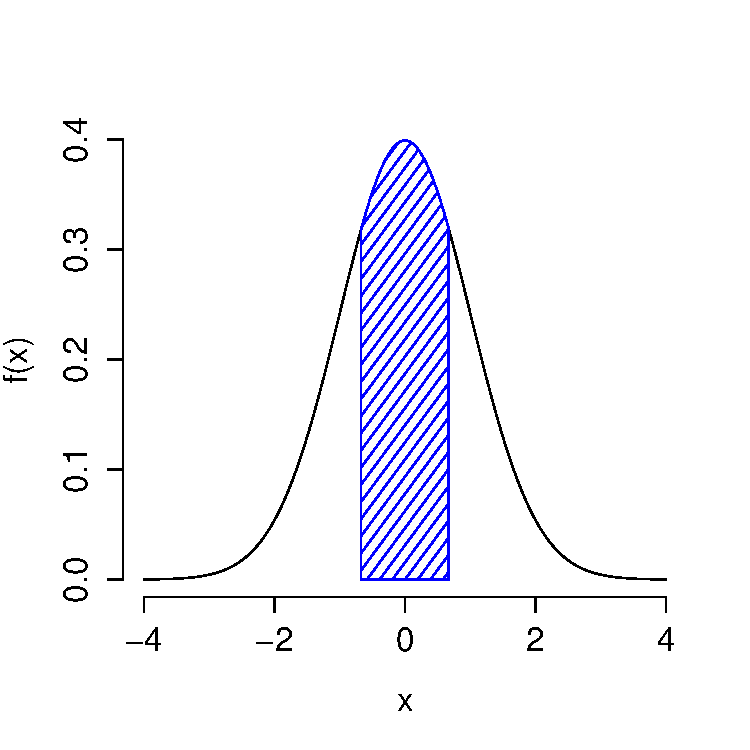
\includegraphics[scale = 0.55]{./images/tail5}
\end{center}
\end{frame}
%%%%%%%%%%%%%%%%%%%%%%%%%%%%%%%%%%%%%%%%
\begin{frame}
\frametitle{95\% Central Interval for Standard Normal \hfill 
\includegraphics[scale = 0.05]{./images/clicker}}

Suppose $X$ is a standard normal random variable. What value of $c$ ensures that $P(-c \leq X \leq c) \approx \alert{0.95}$?

\end{frame}


%%%%%%%%%%%%%%%%%%%%%%%%%%%%%%%%%%%%%%%%

\begin{frame}
\frametitle{R Commands for \emph{Arbitrary} Normal Distributions}
Let $X \sim N(\mu, \sigma^2)$ . Then we can use R to evaluate the CDF and Quantile function of $X$ as follows:
\vspace{1em}
\begin{table}
\centering
\fbox{\begin{tabular}{ll}
CDF $F(x)$&\texttt{pnorm(x, mean = $\mu$,  sd = $\sigma$)}\\
Quantile Function $Q(p)$ & \texttt{qnorm(p, mean = $\mu$,  sd = $\sigma$)}\\
\end{tabular}}
\end{table}
\vspace{1em}
\alert{Notice that this means you don't have to transform $X$ to a standard normal in order to find areas under its pdf using R.}
\end{frame}
%%%%%%%%%%%%%%%%%%%%%%%%%%%%%%%%%%%%%%%%
\begin{frame}
\frametitle{Example from Homework: $X \sim N(0,16)$}

One Way:
			\begin{eqnarray*}
				P(X \geq 10) &=&  1 - P(X \leq 10) = 1 - P(X /4\leq 10/4)\\
				&=& 1 - P(Z\leq 2.5) =   1 - \Phi(2.5) =  1 - \mbox{\texttt{pnorm(2.5)}}\\ 
				&\approx& 0.006
			\end{eqnarray*}
\pause
An Easier Way:
	\begin{eqnarray*}
	P(X \geq 10) &=& 1 - P(X \leq 10)\\ 
	&=&  1 - \texttt{pnorm(10, mean = 0, sd = 4)} \\ 
	&\approx& 0.006
	\end{eqnarray*}
\end{frame}
%%%%%%%%%%%%%%%%%%%%%%%%%%%%%%%%%%%%%%%%

\end{document}
